\documentclass{report}

\usepackage[utf8]{inputenc}
\usepackage[T1]{fontenc}
\usepackage[french]{babel}
\usepackage[]{amsmath}
\usepackage{amsfonts}
\usepackage{mathrsfs}
\usepackage[]{graphicx}
\usepackage{fullpage}
\usepackage[usenames,dvipsnames]{color}
\usepackage{listingsutf8}
\usepackage[hidelinks]{hyperref}

\definecolor{gray}{gray}{0.70}

\lstset{%
	tabsize=4,
	basicstyle=\small\ttfamily,
	numberstyle=\scriptsize\ttfamily,
	texcl=true,
	extendedchars=true,
	inputencoding=utf8/latin1
}

\lstdefinestyle{prog}{%
	caption=Programme,
	numbers=left,
	frame=L,
	language=c,
	tabsize=4,
	basicstyle=\small\ttfamily,
	numberstyle=\scriptsize\ttfamily,
	keywordstyle=\color{BlueViolet},
	stringstyle=\color{Green},
	commentstyle=\color{gray},
	showstringspaces=false
}

\lstdefinestyle{output}{%
	caption=Résultat,
	frame=single,
	belowcaptionskip=1\baselineskip,
	breaklines=true
}

\author{Rémi \textsc{Nicole}}
\title{Rapport du TP 6 d'IGI-2001}
\date{}

\begin{document}

\maketitle

\chapter{Exercice 1}
\lstinputlisting[style=prog]{exo1.c}
\lstinputlisting[style=output]{out1}

\chapter{Exercice 2}
\lstinputlisting[style=prog]{exo2.c}
\lstinputlisting[style=output]{out2}

\section{Question 1}
On doit constater un résultat égal à 0 car les valeurs ont été initialisée à la
déclaration.

\chapter{Exercice 3}
\lstinputlisting[style=prog]{exo3.c}
\lstinputlisting[style=output]{out3}

\chapter{Exercice 4}
\lstinputlisting[style=prog]{exo4.c}
\pagebreak
\begin{figure}[h]
	\centering
	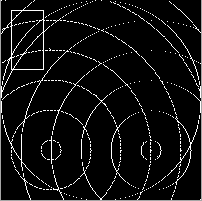
\includegraphics{out4.png}
	\caption{Capture d'écran du résultat de l'exercice 4}
\end{figure}
À gauche les cercles créés avec la méthode trigonométrique et à droite
avec la méthode cartésienne

\section{Question 1}
Ce code initialise le système d'affichage, les couleurs noir et blanc, la
fenêtre, l'affiche, attends la possibilité de dessiner dessus, dessine la
diagonale haut gauche, deux points aux coordonnées $ \begin{pmatrix} 10\\ 50
\end{pmatrix} $ et $ \begin{pmatrix} 10\\ 51 \end{pmatrix} $ et finalement
``force'' l'affichage (autrement dit les affiche).

\section{Question 2}
\subsection{Solution cartésienne}

\paragraph{} Afin de dessiner un cercle, on utilise l'équation cartésienne du
cercle:

\begin{equation}
	{\left(x-x_0\right)}^2 + {\left(y-y_0\right)}^2 = r^2
	\label{cartcercle}
\end{equation}

Avec
$ \begin{pmatrix}
	x_0\\y_0
\end{pmatrix} $
les coordonnées du centre du cercle et $r$ le rayon du cercle.

\paragraph{} Cependant, ne pouvant tracer $y$ sans connaître $x$ ni tracer $x$
sans connaître $y$, il suffit d'isoler la variable $x$ ou la variable $y$ de
l'équation~\ref{cartcercle} pour obtenir une équation exploitable pour le
programme.  On obtient donc:

\begin{equation}
	y = \pm \sqrt{r^2 - {\left(x-x_0\right)}^2} + y_0
	\label{cercle}
\end{equation}

\paragraph{} Le fait d'avoir un $\pm$ dans l'équation~\ref{cercle} n'est en
aucun gênant car il est évidemment possible de calculer les deux possibilités
et de les enregistrer dans le tableau qui sera affiché.

\paragraph{} Malheureusement, la fonction \texttt{pow} de la STL du langage C
gère mal les nombres négatifs à la base. Il faut donc utilise la fonction
\texttt{abs} de la STL pour les valeurs à la base d'une puissance qui risquent
d'être négatives, soit $x-x_0$. L'équation~\ref{cercle} deviendra donc dans le
programme:

\begin{equation}
	y_+ = y_0 + \sqrt{r^2 - {\left|x-x_0\right|}^2}
	\label{progcerclpos}
\end{equation}
et
\begin{equation}
	y_- = y_0 - \sqrt{r^2 - {\left|x-x_0\right|}^2}
	\label{progcerclneg}
\end{equation}

\subsection{Solution trigonométrique}

\paragraph{} Un autre solution serait d'utiliser l'équation paramétrique:

\begin{equation}
	\begin{pmatrix}
		x\\y
	\end{pmatrix}
	=
	\begin{pmatrix}
		r\times\cos(t) + x_0\\
		r\times\sin(t) + y_0
	\end{pmatrix}
	\label{param}
\end{equation}

et de faire varier $t$ sur l'intervalle $\left[0,2\pi\right]$ via une boucle
\lstinline[style=prog]|for| et par étape déterminant la précision du tracé du
cercle.

\subsection{Avantages et inconvénients}

\paragraph{} Les avantages de la solution cartésienne sont d'abords le fait que
l'on puisse déduire deux valeurs à partir d'une seule racine (à une addition
près) et donc dessiner deux valeurs ``en même temps'' et le fait que la
précision sur l'axe x est ``parfaite'' de par le fait que l'on incrémente pixel
par pixel. Cependant, cela entraîne des points manquant par rapport à l'axe y,
ce qui se remarque sur la capture d'écran.

\paragraph{} Les avantages de la solution trigonométrique sont sa simplicité (8
lignes de moins que la solution cartésienne) et le fait qu'il y ait une
précision constante sur les deux axes. Cela entraîne aussi le fait que pour
avoir une précision correcte sur un cercle quelque soit son rayon, il faut
calculer le pas de la boucle \lstinline[style=prog]|for| en fonction du rayon.
Pour cela, il faut que le différence entre deux valeurs adjacente soit
inférieure à $\sqrt{2}$ (la diagonale d'un carré de longueur $1$). On a donc:

\[
	\sqrt{{\left(x(t) - x(t+s)\right)}^2 + {\left(y(t) - y(t+s)\right)}^2} \leq \sqrt{2}
\]

avec $x(t)$ et $y(t)$ les fonctions d'abscisse et d'ordonnée de l'équation
paramétrique~\ref{param} et $s$ l'étape corrélée à la précision du tracé du
cercle qui est utilisé dans la boucle \texttt{for}.

\begin{align*}
	\Leftrightarrow &~{\left(r\times\cos(t) + x_0 - r\times\cos(t+s) - x_0\right)}^2 +
					  {\left(r\times\sin(t) + y_0 - r\times\sin(t+s) - y_0\right)}^2
					& \leq 2\\
	\Leftrightarrow &~{\left(r\times(\cos(t) - \cos(t+s))\right)}^2 +
					  {\left(r\times(\sin(t) - \sin(t+s))\right)}^2
					& \leq 2\\
	\Leftrightarrow &~r^2 \times \left({\left(\cos(t) - \cos(t+s)\right)}^2 +
									   {\left(\sin(t) - \sin(t+s)\right)}^2\right)
					& \leq 2\\
	\Leftrightarrow &~r^2 \times \left({\cos(t)}^2 + {\sin(t)}^2
									   - 2\times\big(\cos(t)\cos(t+s) + \sin(t)\sin(t+s)\big)
									   + {\sin(t+s)}^2 + {\cos(t+s)}^2 \right)
					& \leq 2\\
	\Leftrightarrow &~2\times r^2 \times \left(1 - \big(\cos(t)\cos(t+s) + \sin(t)\sin(t+s)\big)
										 \right) & \leq 2\\
	\Leftrightarrow &~r^2\times\bigg(1 - \Big(\cos(t)\big[\cos(t)\cos(s) - \sin(t)\sin(s)\big]
											 + \sin(t)\big[\sin(t)\cos(s) + \cos(t)\sin(s)\big]\Big)
								\bigg) & \leq 1\\
	\Leftrightarrow &~r^2\times\left(1 - \cos(s)\times\left({\cos(t)}^2 + {\sin(t)}^2\right)\right) & \leq 1\\
	\Leftrightarrow &~r^2\times(1-\cos(s)) & \leq 1\\
	\Leftrightarrow &\cos(s) & \geq 1 - \dfrac{1}{r^2}\\
\end{align*}

et comme $1-\dfrac{1}{r^2} \in [-1,1]$ et que la fonction $\cos^{-1}$ est
décroissante sur $[-1,1]$ on en déduit que:
\begin{equation}
	s \leq \cos^{-1}\left(1-\dfrac{1}{r^2}\right)
\end{equation}

Cependant, on sait que $r$ est petit donc on peut faire un approximation de
$\cos(x)$ en $1-\dfrac{x^2}{2}$. Cela donne:

\begin{align*}
	1-\dfrac{s^2}{2}                    & \geq 1-\dfrac{1}{r^2}\\
	\Leftrightarrow\qquad\dfrac{s^2}{2} & \leq \dfrac{1}{r^2}\\
\end{align*}
Et par approximation de la racine, on obtient donc:
\begin{equation}
	s \leq \dfrac{1.41}{r}
\end{equation}

Ce résultat s'explique aussi par le fait que la différentielle de la
circonférence d'un cercle est égale à:

\begin{equation}
	\partial \mathcal{C} = r\times\partial t \leq \sqrt{2}
\end{equation}

Avec $\mathcal{C}$ la circonférence du cercle et avec $\partial t = s$. Cela
nous donne donc:

\begin{equation}
	s \leq \dfrac{\sqrt{2}}{r} \simeq \dfrac{1.41}{r}
\end{equation}

\paragraph{} On utilise donc cette approximation afin d'avoir une étape
convenable pour la précision du tracé du cercle. Cela fait donc encore un
calcul de plus (mais approximé) par rapport à la méthode cartésienne qui est
dans ce cas de figure.

\end{document}
% vim: spelllang=fr:spell
